%!TEX TS-program = xelatex
%!TEX encoding = UTF-8 Unicode

\documentclass[a4paper]{article}

\usepackage{xltxtra}
\usepackage{amsfonts}
\usepackage{polyglossia}
\usepackage{fancyhdr}
\usepackage{geometry}
\usepackage{dsfont}
\usepackage{amsmath}
\usepackage{amsthm}
\usepackage{amssymb}
\usepackage{physics}
\usepackage{mathtools}
\usepackage{bm}
\usepackage{float}
\usepackage{listings}

\geometry{a4paper,left=15mm,right=15mm,top=20mm,bottom=20mm}
\pagestyle{fancy}
\lhead{Devon Morris}
\chead{Detection \& Estimation Theory - Final Project}
\rhead{\today}
\cfoot{\thepage}

\setlength{\headheight}{23pt}
\setlength{\parindent}{0.0in}
\setlength{\parskip}{0.0in}

\newtheorem*{prop}{Proposition}
\newtheorem*{defn}{Definition}
\newtheorem*{thm}{Theorem}
\newtheorem*{cor}{Corollary}
\newtheorem*{lem}{Lemma}
\newtheorem*{rem}{Remark}

\DeclarePairedDelimiterX{\inn}[2]{\langle}{\rangle}{#1, #2}

\begin{document}
\section*{Part 1: Problem Formulation}%
  The first task is to generate an $\mathbf{R}$. For notational simplicity, let $\text{toep}(\bm{\theta})$, be the toeplitz matrix formed by the vector $\bm{\theta}$. As mentioned in the project handout, it is not sufficient to randomly sample $\bm{\theta}$ and create $\mathbf{R} = \text{toep}(\bm{\theta})$ because $\text{toep}(\bm{\theta})$ is not guaranteed to be positive semi-definite.  Let $\bm{z} \in \mathds{R}^M$, be a randomly sampled vector. Now, note that given any $\bm{x} \in \mathds{R}^M$
  \[
    \bm{x}^\top \text{toep}(\bm{z}) \bm{x} \geq \lambda_{\min} \bm{x}^\top \bm{x},
  \]
  where $\lambda_{\min}$ is the smallest eigenvalue of $\text{toep}(\bm{z})$. Thus giving the relation,
  \[
    \bm{x}^\top \text{toep}(\bm{z}) \bm{x} - \lambda_{\min} \bm{x}^\top \bm{x} \geq 0.
  \]
  If $\lambda_{\min} \geq 0$, then $\text{toep}(\bm{z})$ is positive semi-definite. If $\lambda_{\min} < 0$, then $-\lambda_{\min} = |\lambda_{\min}|$ and the matrix
  \[
  \text{toep}(\bm{z}) + |\lambda_{\min}|\mathbf{I}
  \]
  is positive semi-definite. In this manner, there is a positive semi-definite $\mathbf{R}$ given any random $\bm{z}$. Furthermore, if $\bm{z} = [z_1, z_2, \dots, z_n]^\top$. This then defines $\bm{\theta}$ 
  \[
    \bm{\theta} = 
    \begin{cases}
      [z_1, z_2, \dots, z_n]^\top & \lambda_{\min} \geq 0 \\
    [z_1 + |\lambda_{\min}|, z_2, \dots, z_n]^\top & \lambda_{\min} < 0 \\
    \end{cases}
  \]
  To generate $\bm{X}_k$ samples, simply generate $\mathbf{Y}_k: \mathcal{N}\left( 0, \mathbf{I} \right)$, using \texttt{randn} in matlab and multiply by $\text{toep}(\bm{\theta})^{1/2}$. We will create a data matrix
  \[
    \bm{X} = 
    \begin{bmatrix}
      \bm{X}_1 & \bm{X}_2 & \cdots & \bm{X}_k
    \end{bmatrix}
  \]
  which is just our random samples stacked column-wise.
  \section*{Part 2: Derivation of CRB}%
  Before proceeding, it is useful to note that the definition of fisher information in the given paper and the textbook differ slightly. The $\mathcal{M}$ given in the paper is the fisher information from a single sample and $\mathbf{J}$ in the book takes all samples into account. Thus they differ by the scale factor $N$. We will now show that they are equivalent (up to this scale factor). According to Scharf,
  \[
    \begin{aligned}
      J_{ij} &= \frac{N}{2} \tr \left[ \mathbf{R}^{-1} \pdv{\mathbf{R}}{\bm{\theta}_i}  \mathbf{R}^{-1} \pdv{\mathbf{R}}{\bm{\theta}_j}\right] \\
             &= \frac{N}{2} \tr \left[\pdv{\mathbf{R}}{\bm{\theta}_i}  \mathbf{R}^{-1} \pdv{\mathbf{R}}{\bm{\theta}_j} \mathbf{R}^{-1}\right] \\
             &= \frac{N}{2} \text{vec} \left( \pdv{\mathbf{R}}{\bm{\theta}_i} \right)^\top \text{vec} \left( \mathbf{R}^{-1} \pdv{\mathbf{R}}{\bm{\theta}_j} \mathbf{R}^{-1} \right) \\
             &= \frac{N}{2} \text{vec} \left( \pdv{\mathbf{R}}{\bm{\theta}_i} \right)^\top \left( \mathbf{R}^{-1} \otimes \mathbf{R}^{-1} \right) \text{vec} \left( \pdv{\mathbf{R}}{\bm{\theta}_j}\right) \\
             &=\frac{N}{2} \left( \pdv{\text{vec}(\mathbf{R})}{\bm{\theta}_i} \right)^\top \left( \mathbf{R}^{-1} \otimes \mathbf{R}^{-1} \right) \left( \pdv{\text{vec}(\mathbf{R})}{\bm{\theta}_j}\right) \\
    \end{aligned}
  \]
  It appears according to this derivation that the paper is missing a scale factor of 2. From this, it is straightforward to show that
  \[
    \mathbf{J} = \frac{N}{2}  \left( \pdv{\text{vec}(\mathbf{R})}{\bm{\theta}^\top} \right)^\top \left(\mathbf{R}^{-1} \otimes \mathbf{R}^{-1} \right) \left( \pdv{\text{vec}(\mathbf{R})}{\bm{\theta}^\top} \right)
  \]
  And the cramer rao bound is given by
  \[
    \mathbf{C} = \mathbf{J}^{-1}
  \]
  The crux of this calculation is finding the jacobian. Since $\text{vec}$ commutes with the derivative, lets first analyze $\pdv{\mathbf{R}}{\bm{\theta}_i}$. Let $\left\{\mathbf{e}_i\right\}_{i=1}^M$ be the standard basis for $\mathds{R}^m$. It is easy to see that
  \[
    \pdv{\mathbf{R}}{\bm{\theta}_i} = \text{toep}(\mathbf{e}_i)
  \]
  which implies that
  \[
    \pdv{\text{vec}(\mathbf{R})}{\bm{\theta}_i} = \text{vec}(\text{toep}(\mathbf{e}_i))
  \]
  using this relation, it is easy to see that
  \[
    \pdv{\text{vec}(\mathbf{R})}{\bm{\theta}^\top} = 
    \begin{bmatrix}
      \text{vec}(\text{toep}(\mathbf{e}_1)) &  \text{vec}(\text{toep}(\mathbf{e}_2)) & \cdots & \text{vec}(\text{toep}(\mathbf{e}_M)) 
    \end{bmatrix}
  \]
  where the vecotrs have been column stacked. This is easily calculated in Matlab.
  \section*{Part 3: Sample Vectors}%
  The procedure for generating samples was shown in part 1. See \texttt{final\_proj.m} for an implementation.

  \section*{Part 4: Estimator for $\bm{\theta}$}%
  According to p.260 in Scharf, the MLE estimator of a structure covariance matrix must satisfy
  \[
    \tr \left[ \mathbf{R}^{-1}(\mathbf{R} - \mathbf{S})\mathbf{R}^{-1} \pdv{\mathbf{R}}{\bm{\theta}_i} \right] = 0
  \]
  for all $i$, where $\mathbf{S} = \bm{X}\bm{X}^\top/N$, is the sample covariance. This implies that
  \[
    \tr \left[ \mathbf{R}^{-1}\mathbf{S}\mathbf{R}^{-1} \pdv{\mathbf{R}}{\bm{\theta}_i} \right] = M
  \]
  This math mirrors what was done in part two and the expression
  \[
    \left( \pdv{\text{vec}(\mathbf{R})}{\bm{\theta}^\top} \right)^\top \text{vec}\left( \mathbf{R}^{-1} \left( \mathbf{R} - \mathbf{S} \right) \mathbf{R} \right) = \bm{0}
  \]
  holds.  It turns out that this is a very hard problem to solve analytically, and no analytic solution has been found yet. It can, however, be solved numerically, which I did using \texttt{fsolve} in matlab. By doing it numerically, you can enforce the toeplitz constraint, and you get $\hat{\bm{\theta}}$.


  \section*{Part 5: Sample Estimation Error Variance} 
  Let $T$ denote the number of monte-carlo trials and let $\bm{\theta}_t$ and $\hat{\bm{\theta}}_t$, denote trial $t$. The sample estimation error variance is given by
  \[
    \mathbf{C} = \frac{1}{T} \sum_{t=1}^T (\bm{\theta}_t - \hat{\bm{\theta}}_t)^\top (\bm{\theta}_t - \hat{\bm{\theta}}_t)
  \]
  See \texttt{final\_proj.m} for implementation. I also calculated $\mathbf{C}_S$ as the estimation error covariance of the first column of the sample covariance.

  \section*{Part 6: Plots of CRB vs Estimation Error Variance}%
  Here is the plot comparing the CRB to the error variance of both our estimator and the sample covariance estimator. 
  \begin{figure}[H]
  \begin{center}
    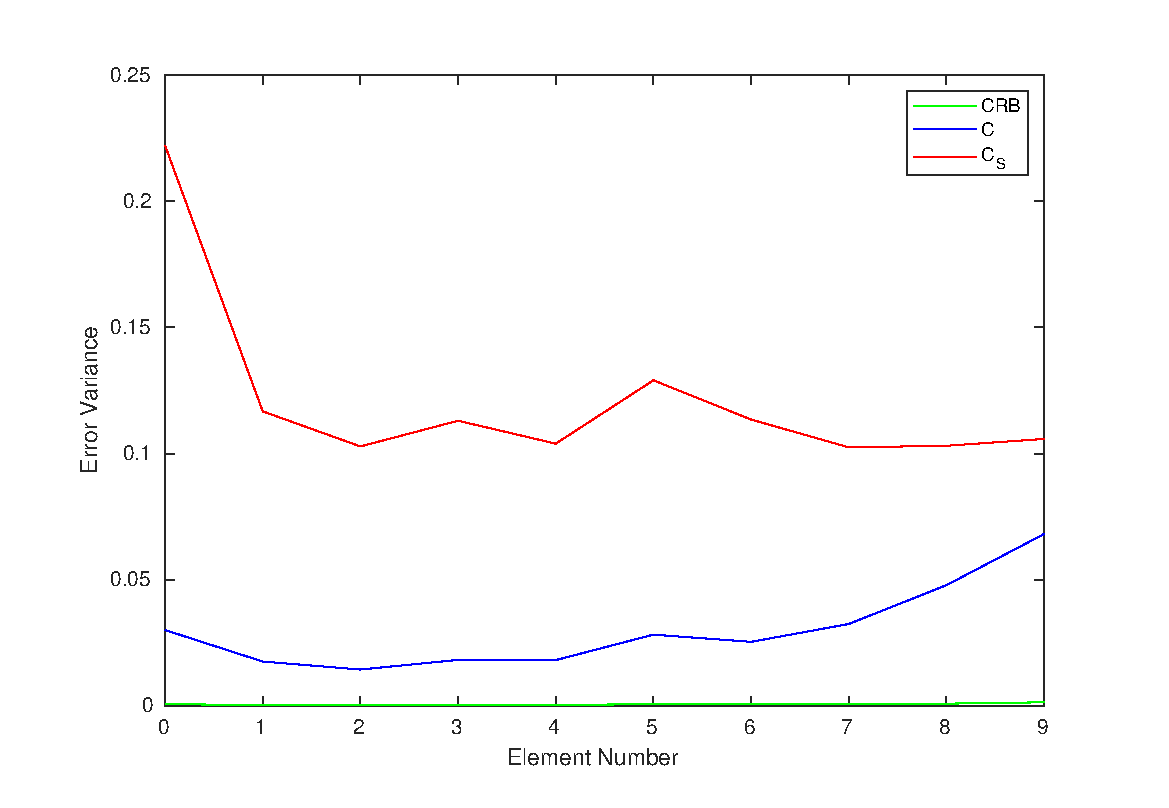
\includegraphics[scale=0.8]{plot_part_6.eps}
  \end{center}
  \caption{Error variance as compared to CRB}
  \end{figure}

  \section*{Part 7: Sensitivity Analysis}%
  To test the sensitivity of our estimator, I generated random noise $\bm{\eta}: \mathcal{N}(0, \sigma_n^2 \mathbf{I})$ and created a new $\bm{\theta}' = \bm{\theta} + \eta$. It turns out that a small bit of unmodeled noise greatly affects the quality of our estimator. When $\sigma_n > 0.01$, the estimator is significantly worse than the sample covariance. I also varied the number of samples $N$. It seems that the estimator needs a minimum of 80 samples to converge properly. Higher number of samples just decreases both the CRB and the estimator variance.

  \section*{Matlab Code:}%
  
 
  I've attached my code as a reference
  \lstinputlisting[language=Matlab]{final_proj.m}

\end{document}
